\subsubsection{Standard behavior}\label{sssec:standard_behavior}
This test aims to address the basic relationship between input current and output voltage. \Cref{tkz:integrator_test} shows the setup used for this test. Channel 8 was used, so the end of the $20\,M\Omega$ resistor is connected to IN[8], and probes are connected to OUT[8] and VBO[8]. 

\begin{figure}[H]
\centering

\usetikzlibrary{shapes,snakes}

\newcommand*{\Vg}{Vg\\ $\color{red}4.5\,V$}
\newcommand*{\Rst}{\textbf{Rst[3]}\\ $\color{blue}reset$} 
\newcommand*{\Res}{Res\\ $\color{red}0.86\,V$}
\newcommand*{\VDD}{VDD3.3\\ $\color{red}3.3\,V$}
\newcommand*{\IN}{$\color{blue}V_{in}$}
\newcommand*{\OUT}{$\color{blue}V_{out}$}
\newcommand*{\VBO}{\color{blue}\textbf{VBO[8]} $\color{red}1.4\,V$}
\newcommand*{\gnd}{gnd\\ $\color{red}0\,V$}
\newcommand*{\C}{$\color{blue}C$}




\tikzstyle{dot} = [draw,shape=circle,fill=black, scale =.3]
\tikzstyle{l_arrow} = [draw,fill = black, regular polygon,regular polygon sides=3, rotate=-90, anchor=south, scale=.5] 
\tikzstyle{l_text} = [anchor=south west]
\tikzstyle{r_arrow} = [draw,fill = black, regular polygon,regular polygon sides=3, rotate=90, anchor=south, scale=.5] 
\tikzstyle{r_text} = [anchor=south east]
\begin{tikzpicture}[scale=1, every node/.style={scale=1}]




\draw[dashed]  (-0.5,5.5) rectangle (0.5,-2);
\node[align=center, anchor=south] at (0,5.5) {voltage\\limiter};

\draw[dashed]  (1.25,5.5) rectangle (5.25,-2);
\node[align=center, anchor=south] at (3.25,5.5) {integrator};

\draw[dashed]  (5.75,5.5) rectangle (9.25,-2);
\node[align=center, anchor=south] at (7.5,5.5) {current mirrors};

%\draw (0,0) to node[nfet]{};

%\draw (0,0) to (mos1.s);
\node(Vg)[nfet, rotate=-90] at (0,2.5) {};
\node[nfet, rotate=-90] (Reset) at (2.5,2) {};
\node[pfet] (CM_H1) at (5,3) {};
\node[nfet] (CM_L1) at (5,-1) {};
\node[nfet] (CM_H2) at (7,3) {};
\node[nfet] (CM_L2) at (7,-1) {};
\node[nfet] (CM_H3) at (9,3) {};
\node[nfet] (CM_L3) at (9,-1) {};



\draw (-1,2.5) node[anchor=east, align=center]{} to (Vg.S);
\draw (Vg.G) |- (0,4.5) node[anchor=south, align=center]{\Vg};
\draw (Vg.B) |- (1,2.5) node[dot]{} |- (CM_H1.G); %top
\draw (1,2.5) |- (1,0.5)  to [C=\C](4,0.5) -| (CM_H1.D);
\draw (1.5,0.5) node[dot]{} -| (1.5,2) |- (Reset.B);
\draw (Reset.G) to (2.5,4.5) node[anchor=south, align=center]{\Rst};
\draw (Reset.D) -| (3.5,0.5) node[dot]{};
\draw (5,0.5) node[dot]{} to (CM_L1.D);
\draw (CM_L1.G) to (4,4.5) node[anchor=south, align=center]{\Res}; 
\draw (CM_L1.S) to (CM_L2.S) to (7,-2.5) node[anchor=north, align=center]{\gnd};
\draw (CM_H1.B) |- (CM_H2.D) to (7,4.5) node[anchor=south, align=center]{\VDD};
\draw (CM_L2.G) |- (4,0) node[dot]{};
\draw (5,0.5) -| (CM_H2.G);
\draw (CM_L1.B) to (CM_L1.S);
\draw (CM_L2.B) to (CM_L2.S);
\draw (CM_H2.B) to (CM_L2.D);
\draw (CM_H3.B) to (CM_L3.D);
\draw (1,3)node[dot]{} |- (8,4) |- (CM_H3.G);
\draw (CM_H3.D) |- (CM_H2.D) node[dot]{};
\draw (CM_L3.S) |- (CM_L2.S) node[dot]{};
\draw (CM_L3.G) |- (6,0) node[dot]{};
\draw (7,1.5)node[dot]{} to (10,1.5) node[anchor=west, align=center]{\OUT};
%\draw (9,1)node[dot]{} to (10,1) node[anchor=west, align=center]{\VBO};

\draw (-2.5,2.5)node[anchor=east, align=center]{\IN} to [R=$20\,M\Omega$](-1,2.5);


\end{tikzpicture}

\caption{Schematic of ROIC channel template}
\label{tkz:integrator_test}
\end{figure}


\Cref{fig:slopes} shows the time versus voltage plot of both the VBO and OUT for a constant input voltage. The rising and falling slopes are the VBO and OUT respecively. The timescale of this plot does not allow for much insight in the behavior of VBO, but it does show some interesting results for the behavior of the integrator. When the reset switches, the input node immediately loses some charge. Note that the oscilloscope matches the rising edge of the reset signal to time is $0\,s$. When the reset is switched, a capacitance is removed almost instantly. It is interesting to observe that the slope immediately after the rising edge of the reset is constant for all input voltages. This means that the observed slope is not limited by the reset transistor, but by the source follower that tries to keep up. This observed slope is therefore the maximum rate at which the output node can be pulled down in the current set-up. Also note that the slope gets steeper when the integrator capacitance decreases. This matches the expected behavior of $\Delta V = \frac{-q}{C}$.


\begin{figure}[h]
    \centering
    \begin{subfigure}[b]{0.475\textwidth}
            \centering
               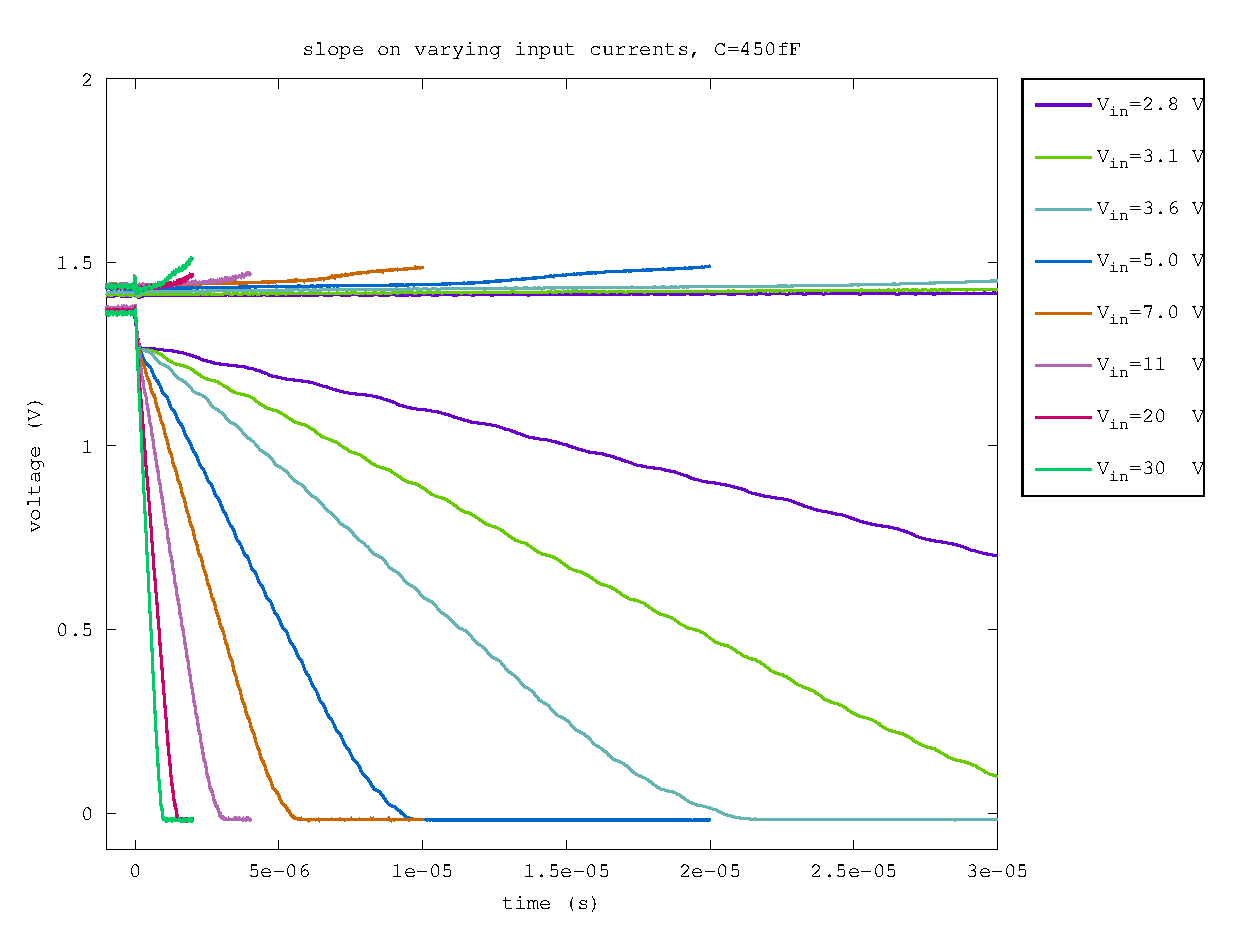
\includegraphics[width=\textwidth]{fig/slope_450fF.eps}
                    \caption[Network2]%
                        {$C0$}    
                            \label{fig:slopes_450fF}
                        \end{subfigure}
                        \hfill
                        \begin{subfigure}[b]{0.475\textwidth}  
                                \centering 
                                    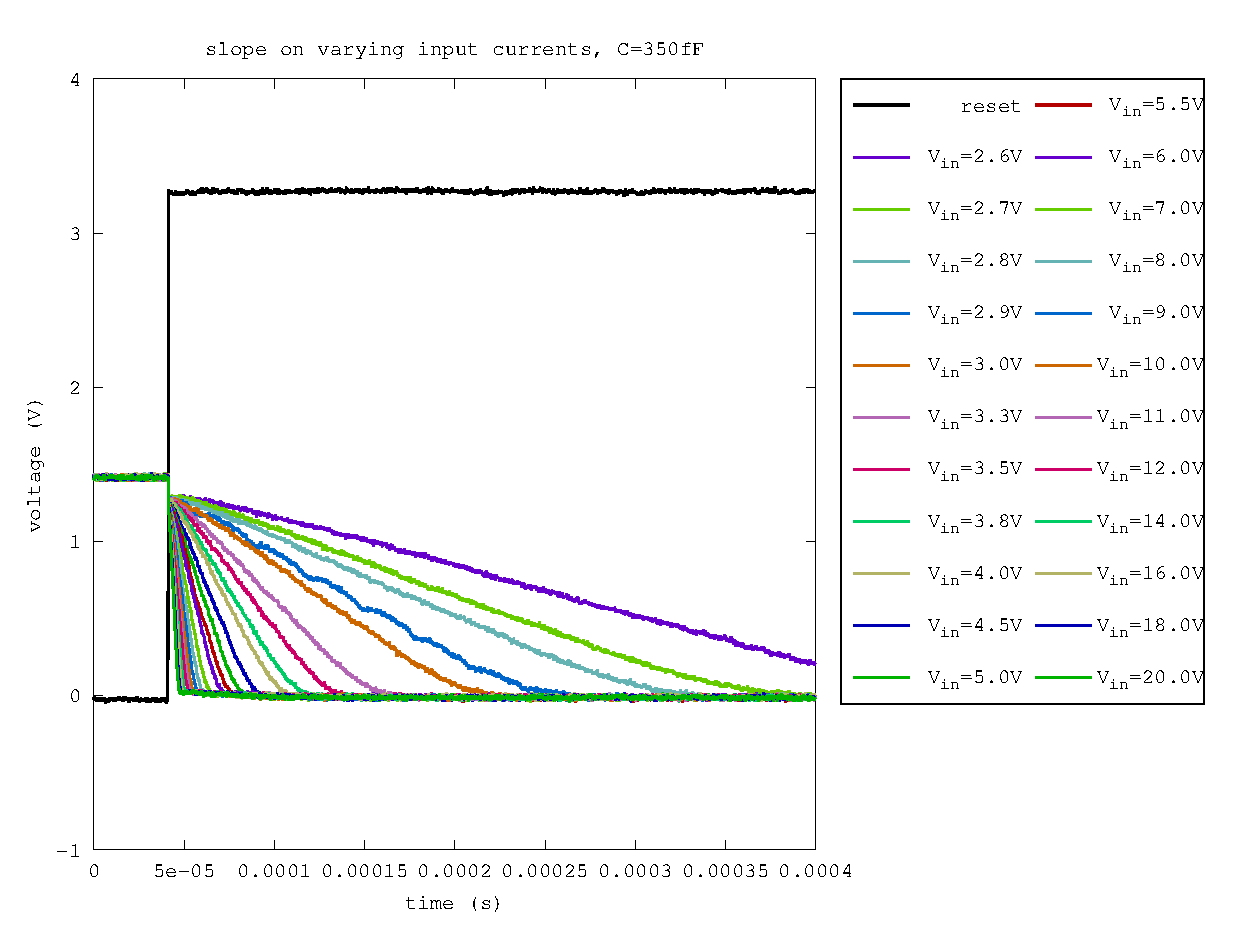
\includegraphics[width=\textwidth]{fig/slope_350fF.eps}
                                    \caption[]
                                        {$C1$}    
                                        \label{fig:slopes_350fF}
                                \end{subfigure}
                            \vskip\baselineskip
                            \begin{subfigure}[b]{0.475\textwidth}   
                                \centering 
                                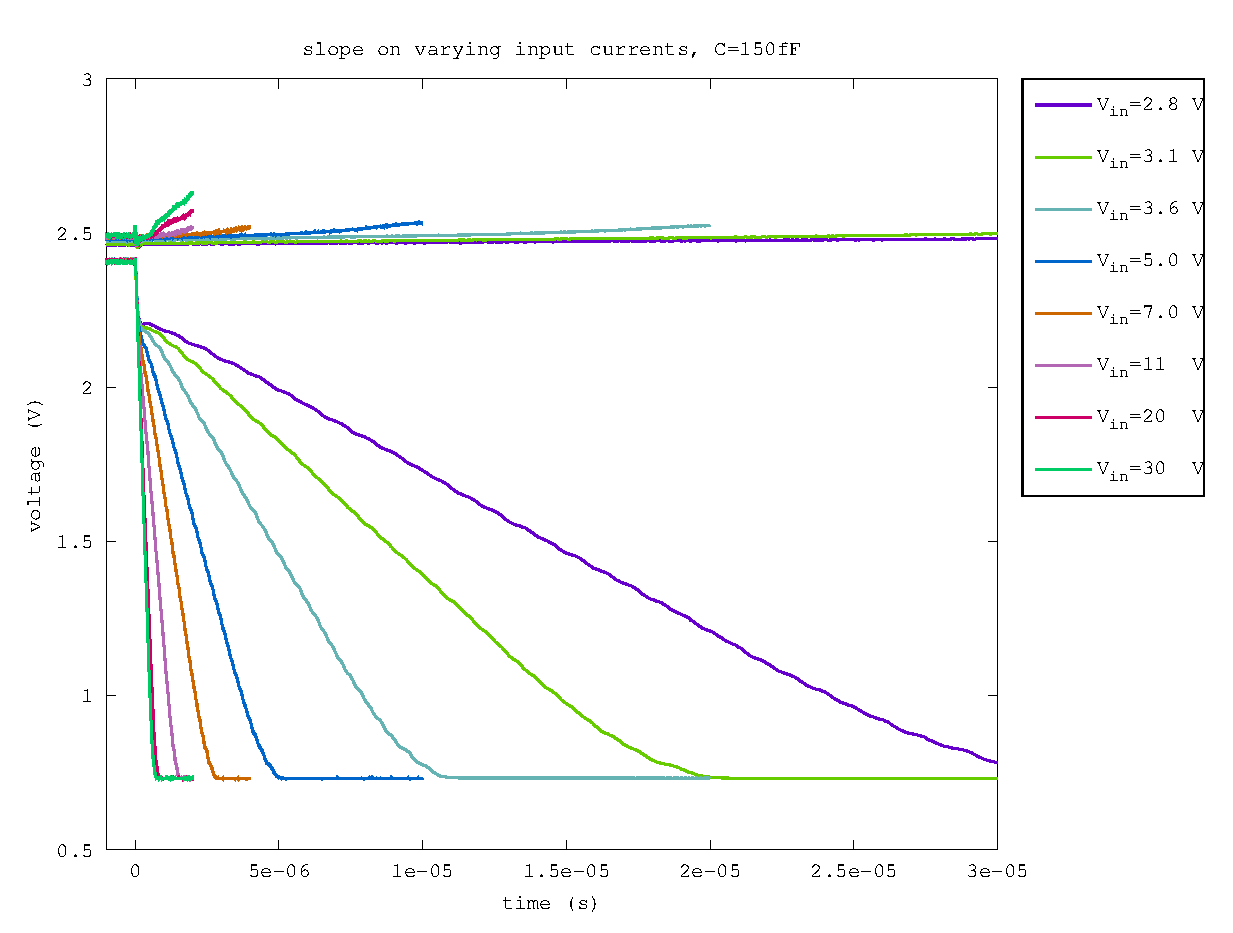
\includegraphics[width=\textwidth]{fig/slope_150fF.eps}
                                \caption[]
                                    {$C2$}    
                                    \label{fig:slopes_150fF}
                            \end{subfigure}
                        \quad
                        \begin{subfigure}[b]{0.475\textwidth}   
                            \centering 
                            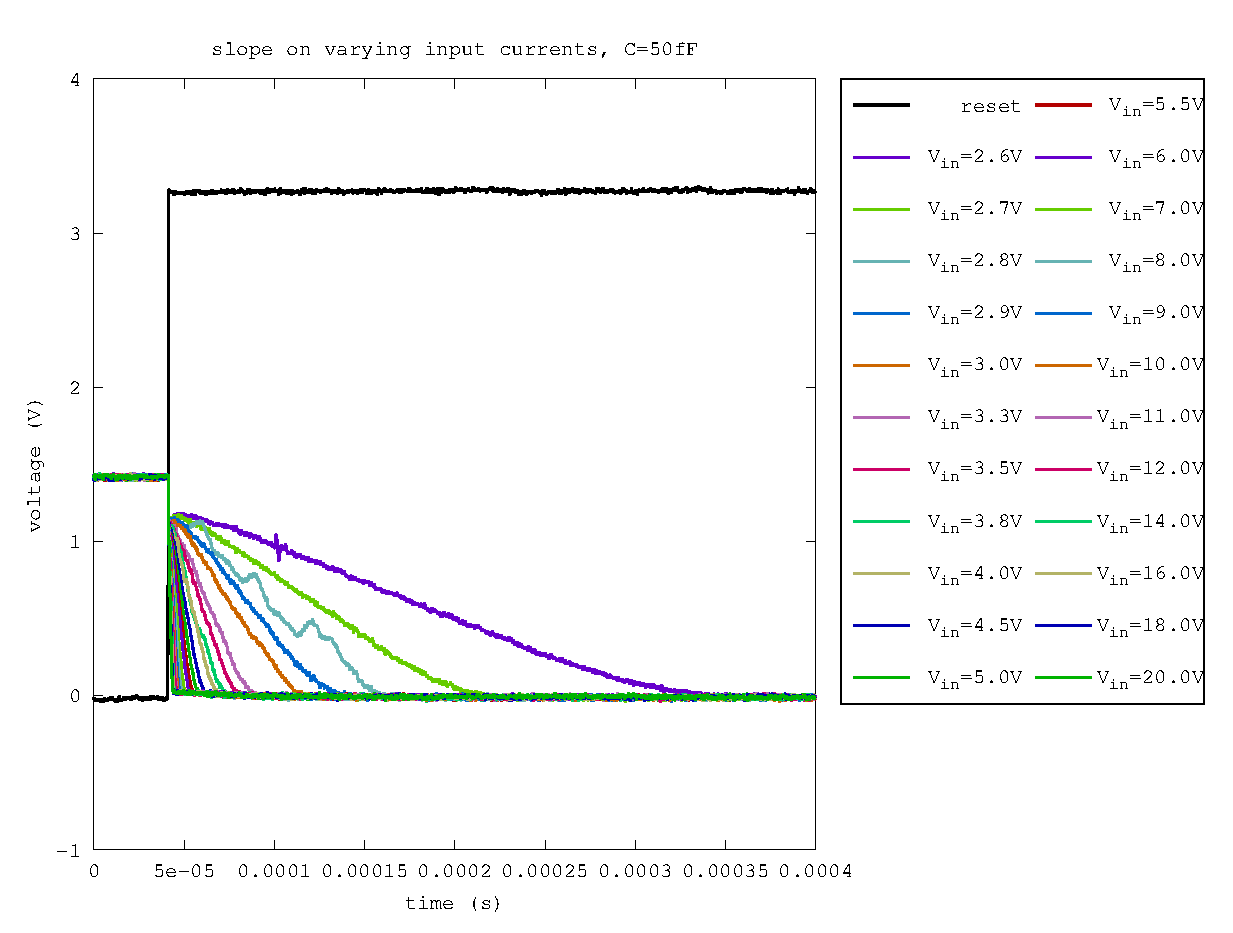
\includegraphics[width=\textwidth]{fig/slope_50fF.eps}
                            \caption[]
                                {$C3$}    
                                \label{fig:slopes_50fF}
                        \end{subfigure}
                    \caption{Expected versus measured charge up times for different input voltages. The input voltage is connected to the input through a resistor of $20\,M\Omega$}
                \label{fig:slopes}
        \end{figure}
    
    \Cref{fig:charges} shows the same plot as \cref{fig:slopes}, but now the x axis is scaled with input current. This shows for \cref{fig:slopes_450fF} and \ref{fig:slopes_350fF} that the relationship between output voltage and charge is equal across different input voltages. For \cref{fig:slopes_150fF} and \ref{fig:slopes_50fF} however, one can see that the higher voltages lose this property. Another intersting observation is that when one looks closely at the plot, one can observe a small oscillation with a period that is constant with charge. Also the period is constant across different voltages. At a later stage it was discovered that serval voltage sources introduced the noise to the system. Removing these devices also removed the observed noise. There was at that point no time left to redo all the measurements however. 


    \begin{figure}[h]
    \centering
    \begin{subfigure}[b]{0.475\textwidth}
        \centering
        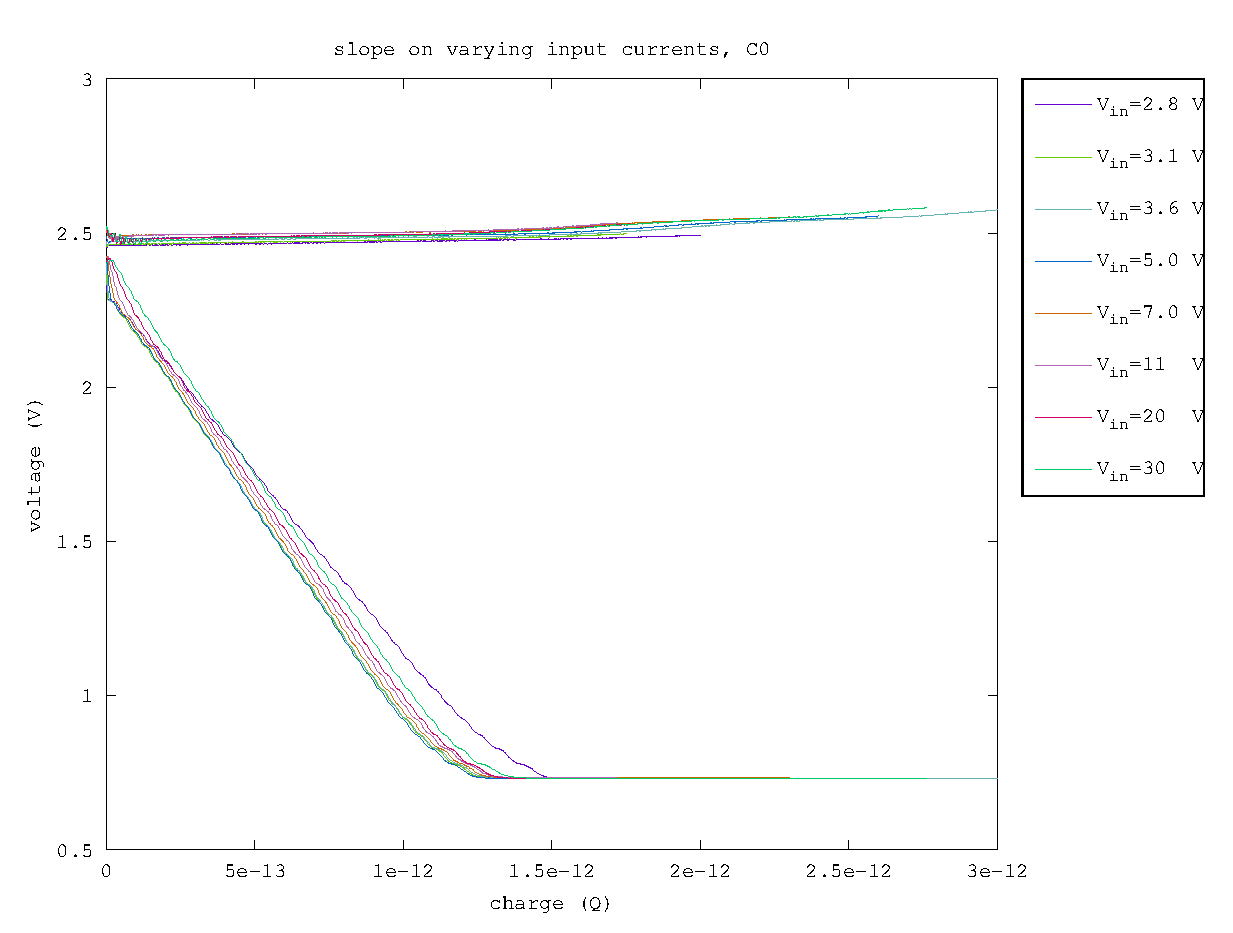
\includegraphics[width=\textwidth]{fig/charge_450fF.eps}
        \caption[Network2]%
        {$C0$}    
        \label{fig:charges_450fF}
\end{subfigure}
\hfill
\begin{subfigure}[b]{0.475\textwidth}  
    \centering 
    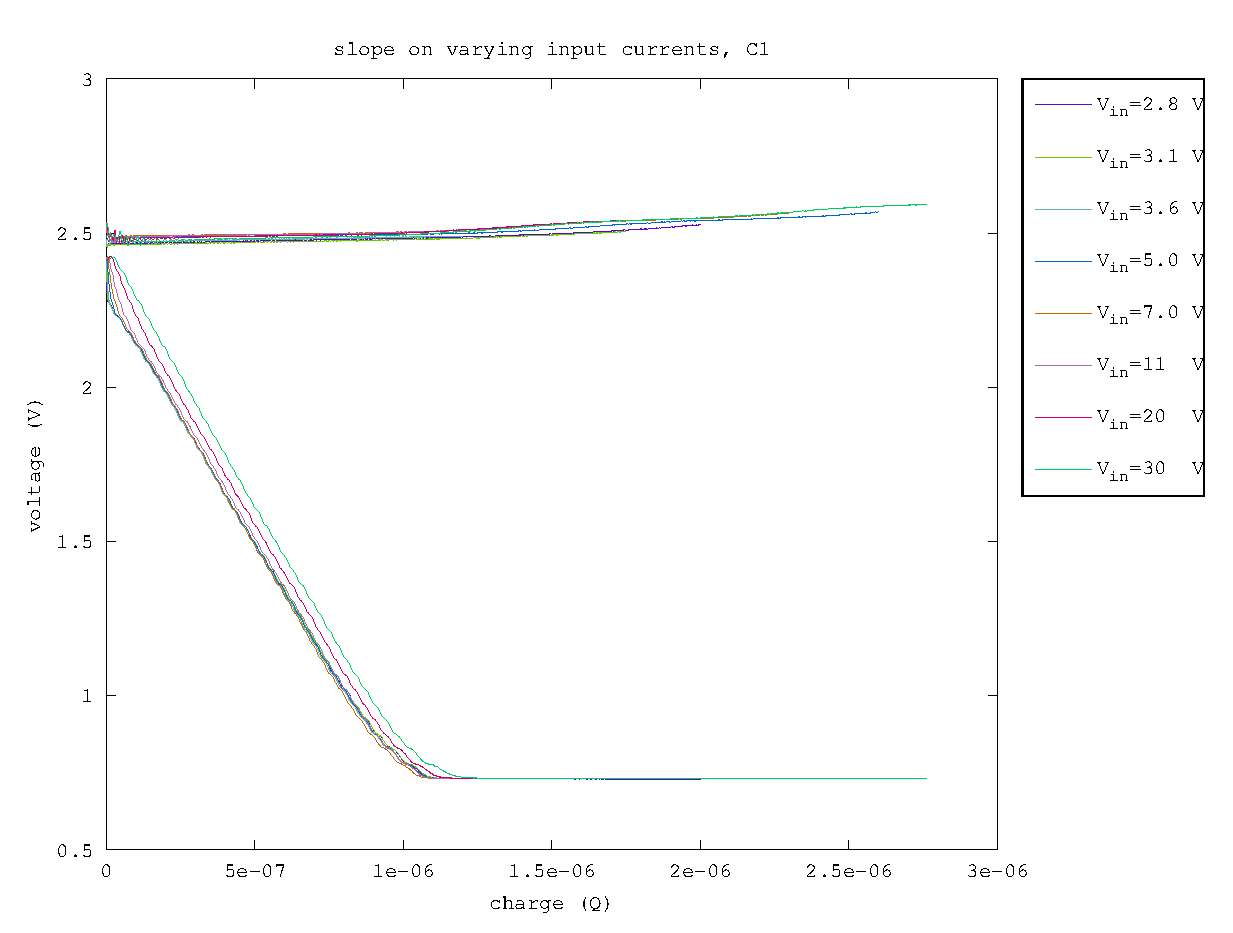
\includegraphics[width=\textwidth]{fig/charge_350fF.eps}
    \caption[]
        {$C1$}    
        \label{fig:charges_350fF}
\end{subfigure}
\vskip\baselineskip
\begin{subfigure}[b]{0.475\textwidth}   
    \centering 
    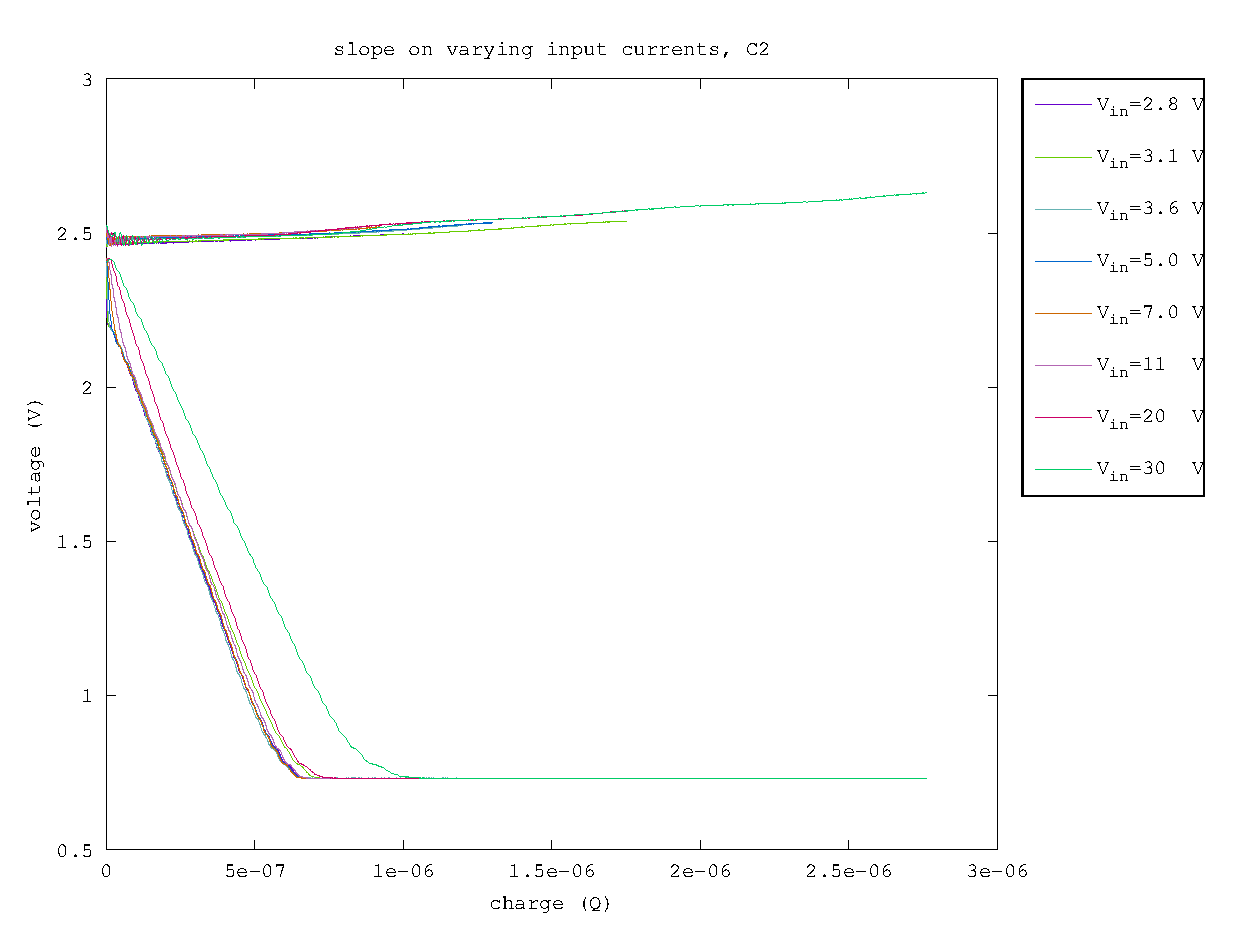
\includegraphics[width=\textwidth]{fig/charge_150fF.eps}
    \caption[]
        {$C2$}    
        \label{fig:charges_150fF}
\end{subfigure}
\quad
\begin{subfigure}[b]{0.475\textwidth}   
    \centering 
    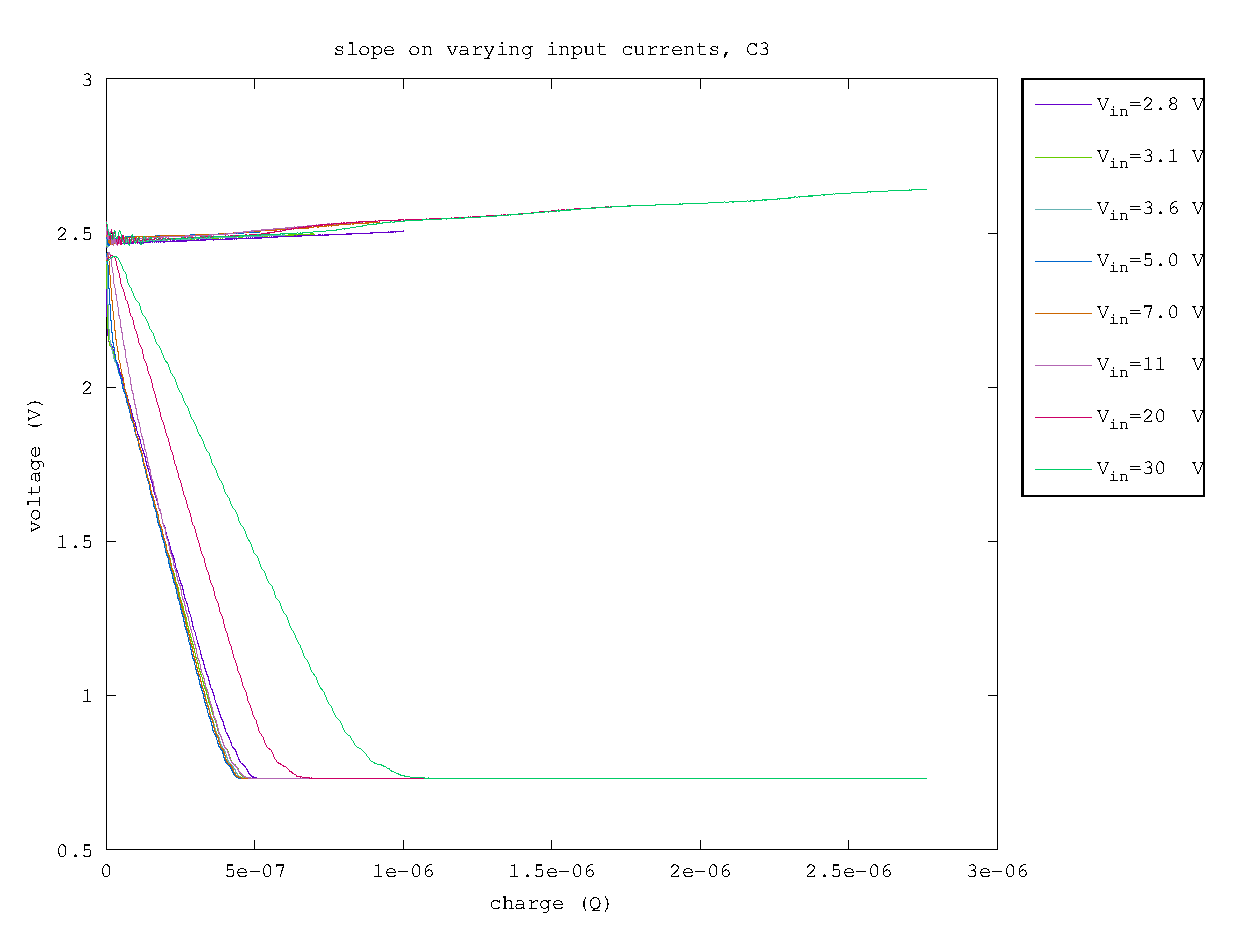
\includegraphics[width=\textwidth]{fig/charge_50fF.eps}
    \caption[]
        {$C3$}    
        \label{fig:charges_50fF}
\end{subfigure}
\caption{This plot is showing charge versus voltage}
\label{fig:charges}
\end{figure}

\Cref{fig:d_slopes} shows the $\delta Q/\delta V$ against charge plots. Note that $\delta Q/\delta V$ is the capacitance. One can observe that while the capacitance is charging, the full value of the capacitancec can be observed, and when the capacitance is comopletely decharged, it behaves as if it is not there. One can use these plots to estimate the integration capacitance. The capitance for \cref{fig:charges_450fF}, \ref{fig:charges_350fF}, \ref{fig:charges_150fF} and \ref{fig:charges_50fF} are approxiately $400\,fF$, $350\,fF$, $200\,fF$ and $150\,fF$ respectively. These values are used for all calculations that involve the integrationcapacitance troughtout the rest of the report.


\begin{figure}[h]
\centering
\begin{subfigure}[b]{0.475\textwidth}
    \centering
    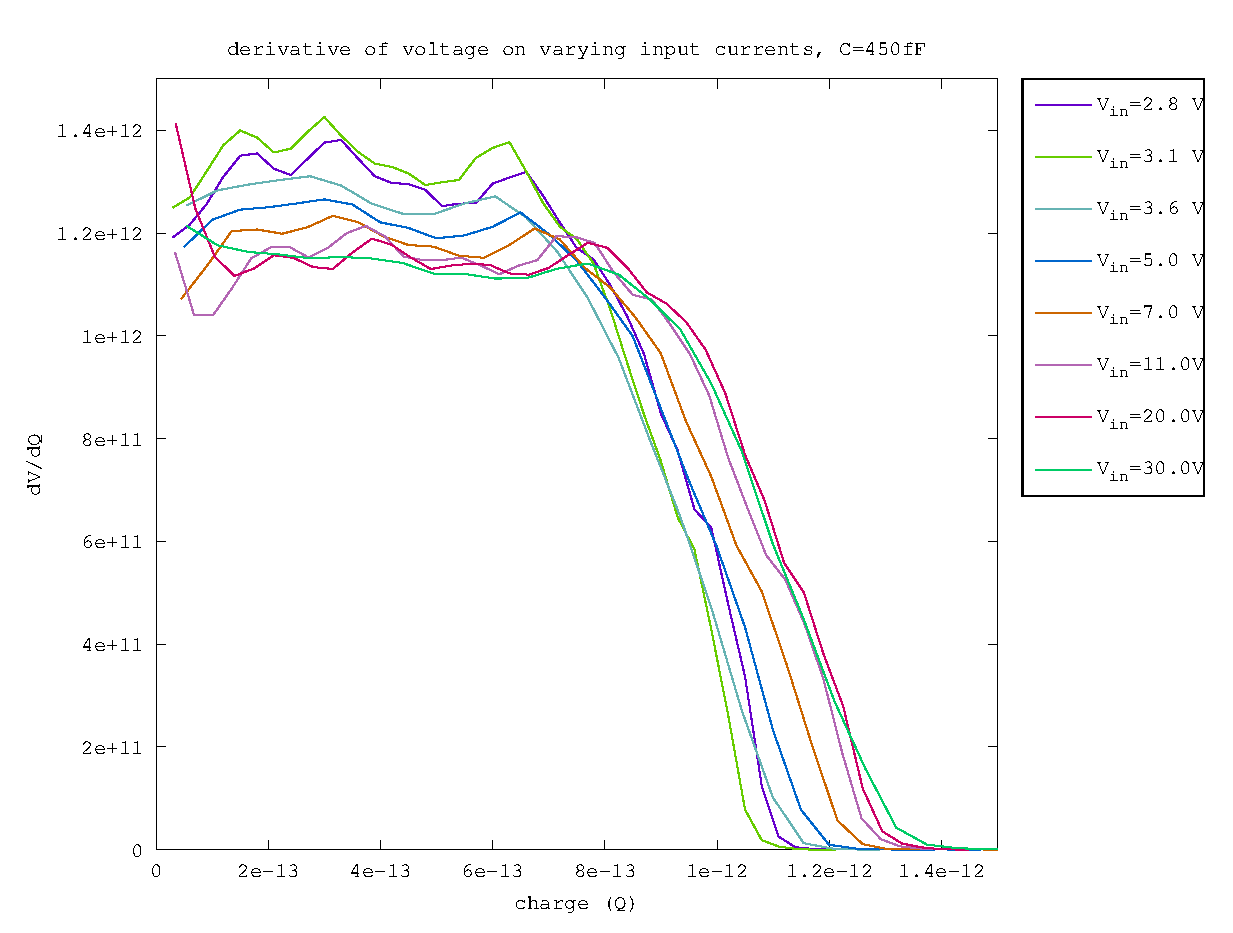
\includegraphics[width=\textwidth]{fig/d_slope_450fF.eps}
    \caption[Network2]%
    {$C0$}    
    \label{fig:d_slopes_450fF}
\end{subfigure}
\hfill
\begin{subfigure}[b]{0.475\textwidth}  
    \centering 
    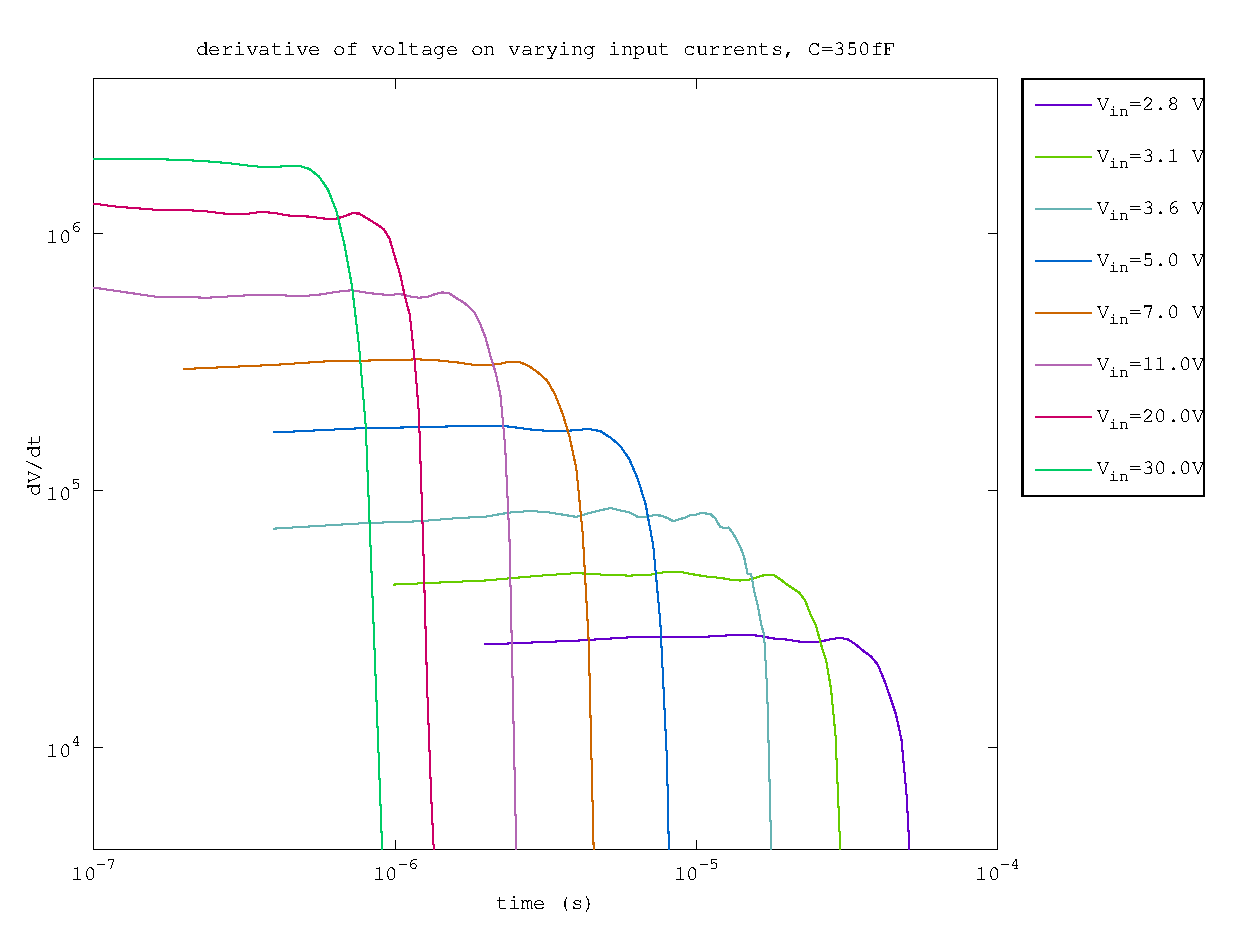
\includegraphics[width=\textwidth]{fig/d_slope_350fF.eps}
    \caption[]
        {$C1$}    
        \label{fig:d_slopes_350fF}
\end{subfigure}
\vskip\baselineskip
\begin{subfigure}[b]{0.475\textwidth}   
    \centering 
    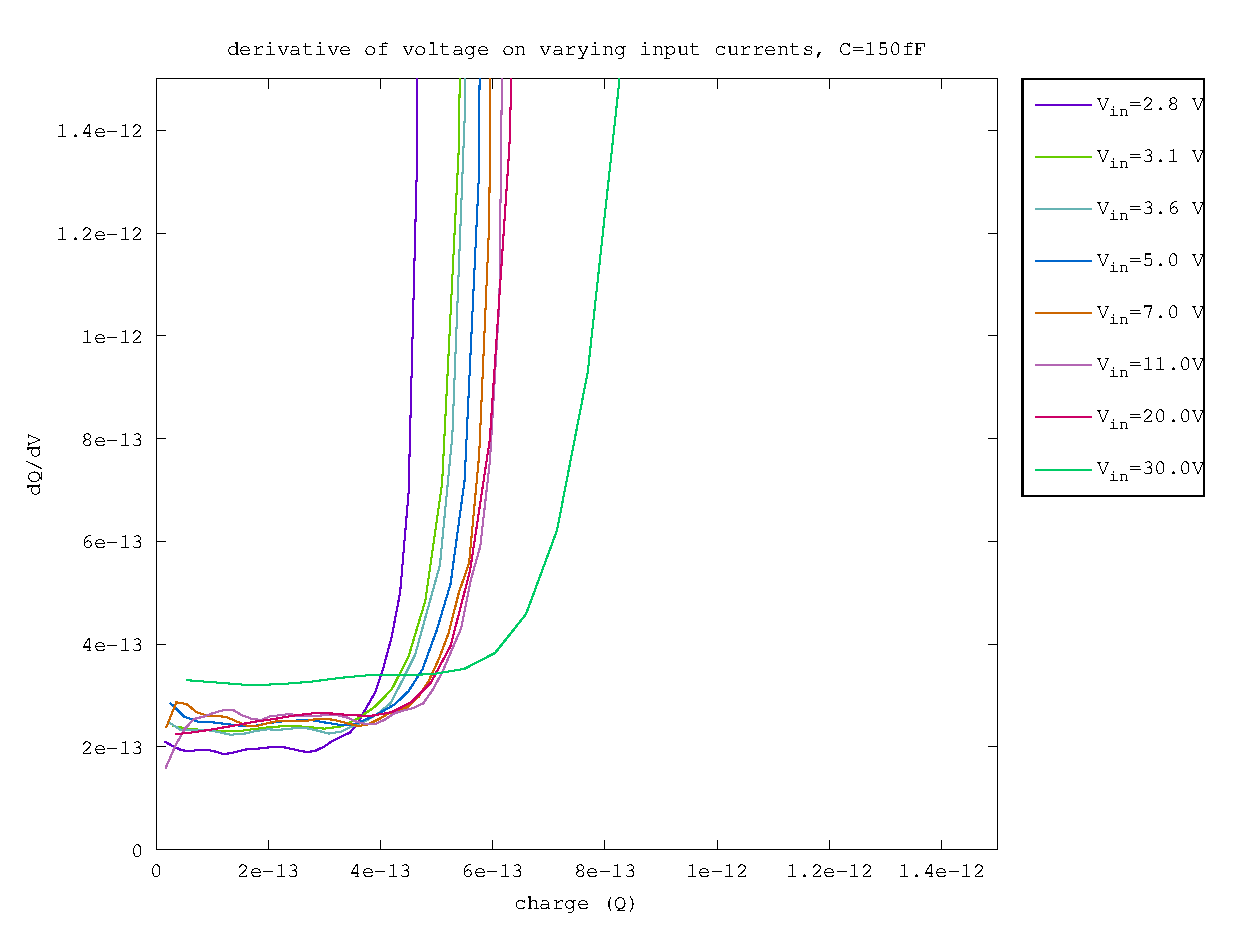
\includegraphics[width=\textwidth]{fig/d_slope_150fF.eps}
    \caption[]
        {$C2$}    
        \label{fig:d_slopes_150fF}
\end{subfigure}
\quad
\begin{subfigure}[b]{0.475\textwidth}   
    \centering 
    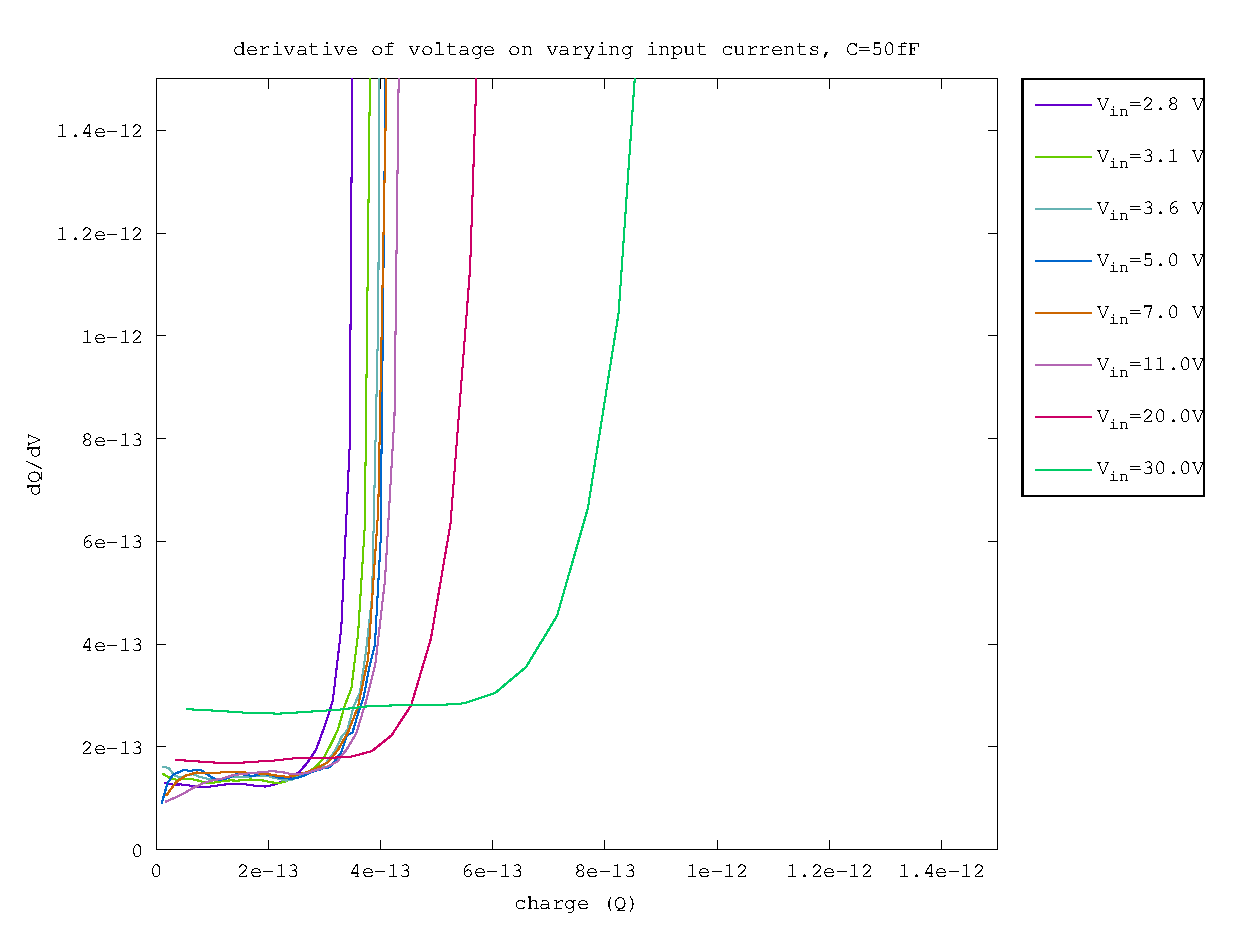
\includegraphics[width=\textwidth]{fig/d_slope_50fF.eps}
    \caption[]
        {$C3$}    
        \label{fig:d_slopes_50fF}
\end{subfigure}
\caption{The plot shows dv/dt against time. The plot is in log scale, which allows for an easy read on the maximum slope and the time needed to discharge the integrator capacitance. }
\label{fig:d_slopes}
\end{figure}



\Cref{fig:e_vs_m} shows $\delta V / \delta t$ against input voltage for all capacitances. One can observe that all four have different slopes at first, but there appears to be a trend that they all converge to a value of $\delta V/\delta t \approx 3.2\cdot10^6$.


\begin{figure}[h]
    \centering
    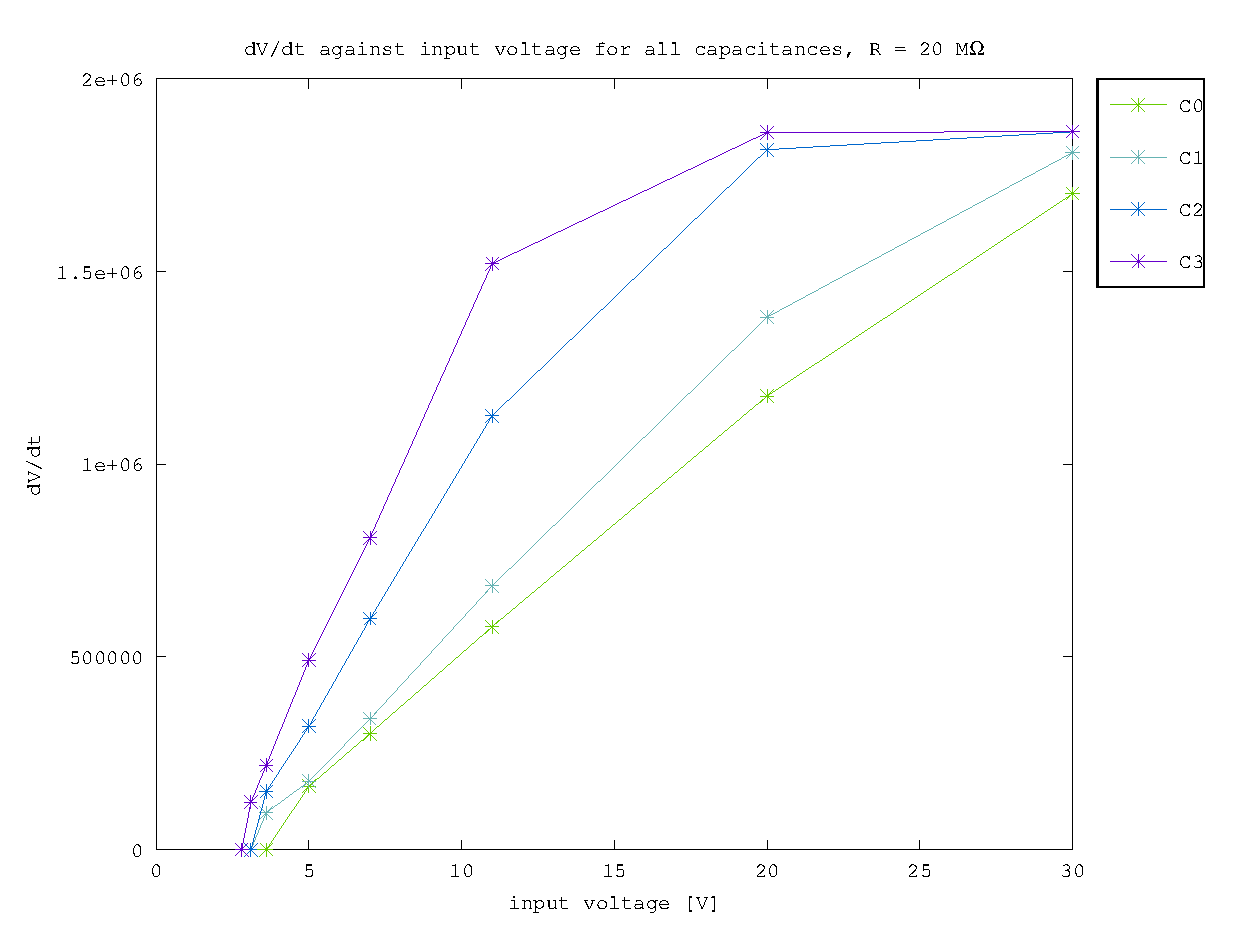
\includegraphics[width=\textwidth]{fig/vin_vs_time_sat.eps}
    \caption[]
        {dV/dt against input voltage for all four capacitances. The x indicate the measurements.}    
        \label{fig:e_vs_m}
\end{figure}

\clearpage
